\documentclass[]{article}
\usepackage[utf8]{inputenc}
\usepackage{graphicx}
\usepackage{amsmath}
\usepackage{amsfonts}
\usepackage{amssymb}
\usepackage{subcaption}
%opening
\title{Homework 2}
\author{Ian Hunt-Isaak}
\date{}
\begin{document}

\maketitle


\section{Introduction}
The continuity equation:
\begin{equation}
\frac{\partial}{\partial t} \varphi + \nabla(\varphi \vec{u}) = 0,
\label{eq:continuity}
\end{equation}
with $\varphi$ the value of interest and $\vec{u}$ the velocity field,  is a special case of a conservation equation, in which there are no diffusion or source terms. are those that describe the transport of some physical quantity. This equation describes the flow of an incompressible fluid, such as water, and therefore is a highly useful equation to be able to solve numerically. Unfortunately even something as simple as the continuity equation, Eq. \ref{eq:continuity}, can be incredibly difficult to approach numerically. In simulating this we have the familiar constraint of stability, i.e. that the solution values will not explode, and we also require that our values be positive for all time and space. This latter requirement comes from the fact that when simulating mass transport it would be physically meaningless to have negative matter. 

Without a diffusive term however we can begin to see wiggles in our solution on account of the very short wavelength required by a sharp edge to a waveform. So if you were to propogate a square wave the edge of the waveform would require infinitely small wavelengths to properly characterize, unfortunately due to the finite simulation grid size we will necessarily cut out important short wavelengths. 

In this document we will explore the different results from propagating a square wave under Eq. \ref{eq:continuity} via the schemes of Upwind, Lax-Wendroff, Flux Corrected Transport (FCT), FCT + Antidiffusion, and SHASTA a method developed by Boris and Book \cite{shasta}. These algorithms each have their pros and cons and provide different levels fidelity to the analytic solution of an advecting square wave.




\section{Numerical Methods}
In 1-D there are ways to discretize the derivatives in Eq. \ref{eq:continuity}, with the most obvious being the centered difference or upwind approaches. Unfortunately in the case of the purely advective system we are considering the centered difference method will lead to an unstable solution. This could be considered to arise from the fact that in order to do this there is an asymmetry to the order of the time and space derivatives. 

Here we will consider the propagation of an initial square waveform and benefits of several different numerical methods.

\subsection{Upwind}

The stability of the solution for the upwind time marching scheme will be determined by the CFL number with $\frac{u \Delta t}{\Delta X}\leq 1$. With a constant velocity field $u(x) = const$, $\Delta t$ and $\Delta X$ could be chosen such that $\frac{u \Delta t}{\Delta X} =  1$. In this situation the square wave shape will be properly propagated, however if we were to introduce other processes or have a non uniform velocity field then this would no longer work. So for this work we consider the upwind system $\frac{u \Delta t}{\Delta X} < 1$ so as to showcase the diffusivity that would necessarily occur in the other situations. 
\subsection{Lax-Wendroff}
The Lax-Wendroff takes the Upwind method and adds an artificial  velocity dependent diffusive term to counter the numerical diffusivity introduced in the Upwind scheme. This diffusion term has magnitude $\frac{U^2 h}{2} \partial_x^2$. As seen in the results section this does dramatically reduce the numerical diffusivity of the solution, it has the unfortunately side effect of introducing strong dispersive wiggles to the solution. 
\subsection{Flux Corrected Transport (FCT)}
In general FCT methods refer to two step methods. The first step is to propagate the solution in time, even if it means moving off the simulation grid, then to interpolate the new magnitudes back onto the simulation grid. The second step would then be to correct for numerical errors via a balancing of the fluxes between neighboring points. In this document these corrections will be considered in the FCT + Antidiffusion, and SHASTA sections. We will refer to FCT as just the first step of this process

The FCT method unfortunately introduces a strong numerical diffusion, and in the limit of constant U can be viewed as the Lax-Wendroff solution with a strong numerical diffusion with $D = \frac{1}{8}$. So on its own this step is not particularly useful as we will see even stronger diffusion than the Upwind scheme.

\subsection{FCT + Antidiffusion}
The second step, or the correction step, of FCT could be very simply performed by adding an antidiffusive term to FCT first step. To do so we need to consider the fluxes $f$ into the point under consideration from the grid points on either side. That is we will consider:
\begin{equation}
f^n_{j+\frac{1}{2}} = \varphi^n_{j+1}-\varphi^n_{j-1},
\end{equation}
and 
\begin{equation}
f^n_{j-\frac{1}{2}} = \varphi^n_{j}-\varphi^n_{j}.
\end{equation}

We can then find the corrected magnitude as $\bar{\varphi}^{n+1}_j = \varphi_j^n + D\cdot \left(f^n_{j-\frac{1}{2}}-f^n_{j+\frac{1}{2}}\right),$ where D = $-\frac{1}{8}$ to counter the diffusion introduced in the first step.  
\subsection{SHASTA}
As presented by Boris and Book \cite{shasta} the SHASTA algorithm is very similar to the Flux Corrected Transport with explicit $\frac{1}{8}$ antidiffusion. However, instead of simply subtracting an antidiffusive quantity of equal magnitude to the diffusion introduced by the FCT scheme Boris and Book design a correction that prevents the creation of new local extrema. As in the antidiffusion the first step of FCT the correction is:
\begin{equation}
\bar{\varphi}^{n+1}_j = \varphi_j^{n+1} + f^c_{j-\frac{1}{2}}-f^c_{j+\frac{1}{2}},
\end{equation}
where $\bar{\varphi}^n_j$ is the corrected value and the $f^c$ are defined below so as to prevent the creation of local extrema.The difference is in the definition of the correcting fluxes. With $\Delta_{j+\frac{1}{2}} = \varphi^n_{j+1} - \varphi^n_{j}$, $\Delta_{j-\frac{1}{2}} = \varphi^n_{j} - \varphi^n_{j-1}$, and $\Delta_{j\pm\frac{3}{2}}$ defined similarly we can define $f^c$ as follows:

\begin{equation}
f^c_{j+\frac{1}{2}} = sgn(\Delta_{j+\frac{1}{2}}) \text{Max}\left(0,\text{Min}\left(\Delta_{j-\frac{1}{2}} sgn(\Delta_{j+\frac{1}{2}}), \frac{1}{8}|\Delta_{j+\frac{1}{2}}|,\Delta_{j+\frac{3}{2}} sgn(\Delta_{j+\frac{1}{2}}\right)\right)
\label{eq:def_fc_right}
\end{equation}
This equation considers where "mass" could have gone from, or come into point $j$ due to numerical diffusion. It then selects the smallest possible correction with a sign chosen based on the relative magnitudes of $\varphi^n_{j+1}$ and $\varphi^n_{j}$. While, Boris and Book do not provide an equation for $f^c_{j-\frac{1}{2}}$ by considering the intention of how the correction term works we can construct it as follows:

\begin{equation}
f^c_{j-\frac{1}{2}} = sgn(\Delta_{j-\frac{1}{2}}) \text{Max}\left(0,\text{Min}\left(\Delta_{j+\frac{1}{2}} sgn(\Delta_{j-\frac{1}{2}}), \frac{1}{8}|\Delta_{j-\frac{1}{2}}|,\Delta_{j-\frac{3}{2}} sgn(\Delta_{j-\frac{1}{2}}\right)\right).
\label{eq:def_fc_left}
\end{equation}
This construction of $f^c_{j-\frac{1}{2}}$ is the only one that maintains the symmetry of the corrective equation, simply shifting the subscript values by -1 would not be result in proper correction to the FCT method. 

\section{Results}
A square waveform being advected to the right was simulated using the upwind, Lax-Wendroff, Flux Corrected Transport(FCT), FCT + Antidiffusion, and the FCT + Boris and Book correction methods. A comparison of the results of each of these methods can be seen in Figures \ref{fig:constU_f_compare}, and \ref{fig:constU_f_compare_offset}. As expected the upwind scheme does not induce wiggles in the solution, however it does suffer from a numerical diffusion causing the initial square waveform to degrade into a Gaussian waveform. For the upwind solution at least if the $\Delta t$ and $\Delta x$ had been chosen so as such that $\frac{\Delta x}{\Delta t} = U $ the solution would have propogated a perfect square wave. In previously studied systems, such as ADR, this would have led to instability, however, in this case with no physical diffusion we can allow such discretized steps without instability. If however, we had a non uniform velocity field then this would not longer be a viable option and the upwind solution would suffer from the same numerical diffusivity seen here with non optimally chosen time and space steps. The pure FCT scheme without any diffusion correction does see the strongest numerical diffusion, as a consequence of the 1/8 artificial diffusion. The Lax-Wendoff scheme solves the issue of diffusion but induces large wiggles as expected, and does not maintain the positivity of the solution. If we correct the FCT by adding an explicit antidiffusive term with magnitude 1/8 we see that it is indeed similar to the Lax-Wendroff solution, with minimal diffusion but also with greatly reduces wiggles, unfortunately this still does not preserve positivity. Finally, the SHASTA method developed by Boris and Book does the best job of maintaining the square waveform. There are no unphysical wiggles in the solution, and diffusion is minimized. In fact, in Figure \ref{fig:constU_compareH} we can use the diagnostic $H_2$ as a method to compare the numerical diffusivity of the various methods of solution. When we do so we see that the SHASTA method has dramatically less diffusion than either upwind or pure FCT. While it does have more numerical diffusivity than either Lax-Wendroff or FCT + Antidiffusion it has the edge on them in terms of maintaining positivty and consequently is the clear best method of those considered for studying the advection of a square waveform under the continuity equation. 

An unfortunate consequence is that I found that SHASTA takes significantly longer to run than the Upwind scheme scheme, and also markedly more time than Lax-Wendroff and even the slightly less complex FCT + Antidiffusion scheme. 


\begin{figure}
		\centering
		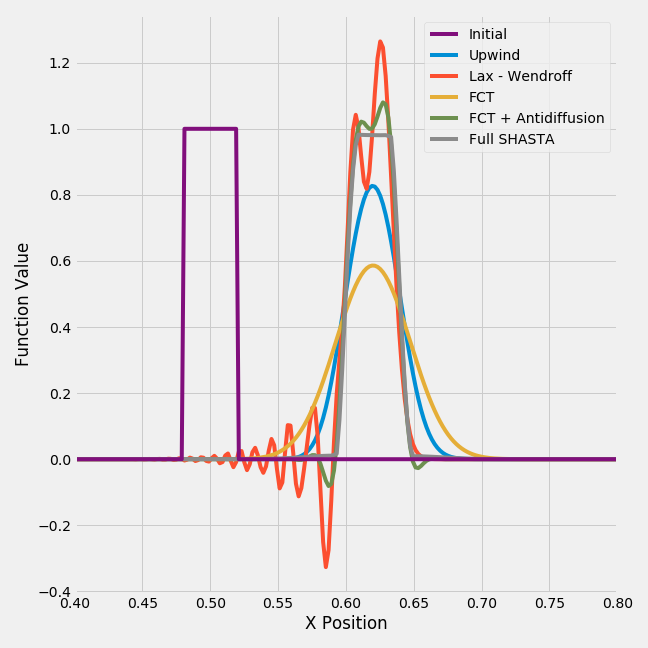
\includegraphics[width=.8\linewidth]{figures/constU_fCompare.png}

	\caption{Comparison of the different approaches to numerically solving Eq. \ref{eq:continuity}. In this comparison we can see that the center of mass is propagated at the same velocity regardless of the time marching method or corrective diffusion steps used. For an easier comparison of profile shapes consider Figure \ref{fig:constU_f_compare_offset}. }
	\label{fig:constU_f_compare}
\end{figure}
\begin{figure}
	\centering
	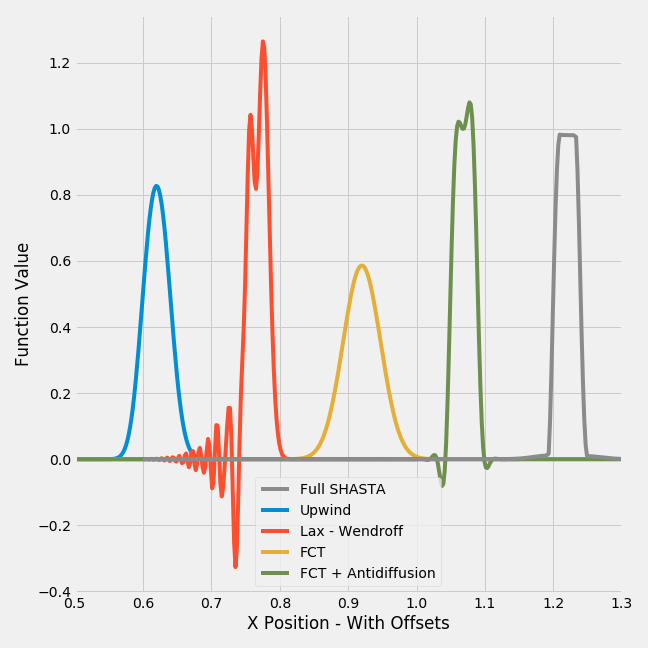
\includegraphics[width=.8\linewidth]{figures/constU_fCompare_offset.png}
	\caption{Comparison of the different approaches to numerically solving Eq. \ref{eq:continuity} after 600 time steps with an initial wave form of a square wave. In this comparison the waveforms have been offset in X from each other so as to compare their shape. Overall the results of this comparison are as expected, with both the Upwind and FCT methods showing strong dispersion, Lax-Wendroff ad FCT + Antidiffusion maintaining the basic square wave shape, but with wiggles, and finally the SHASTA method developed by Boris and Book providing the most accurate results. A comparison of the level diffusion in each method can be seen in Figure \ref{fig:constU_compareH}. }
	\label{fig:constU_f_compare_offset}
\end{figure}
\begin{figure}

		\centering
		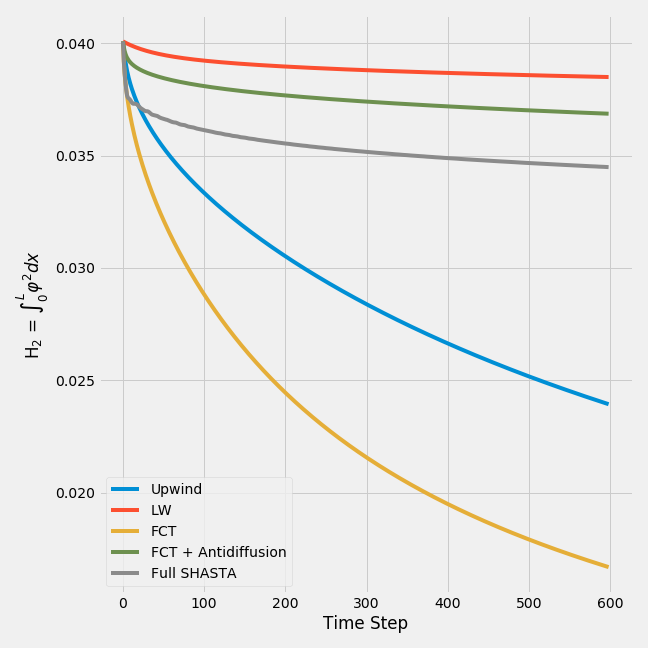
\includegraphics[width=.8\linewidth]{figures/constU_compareH.png}
		\caption{Comparison of the quantity $H_2$, which serves as a measure of the localization (or entropy) of the solution. In this case we can use this as a proxy measure for the amount of numerical diffusion introduced by our solution method, with lower values of $H_2$ corresponding to greater amounts of diffusion. The results here agree with visual inspection of Figure \ref{fig:constU_f_compare_offset}, though they provide a more quantitative sense of the differences of diffusion in the methods. While the SHASTA method is unquestionably the most accurate we can see here that while avoiding wiggles, it does less well than Lax-Wendroff or FCT+Antidiffusion at preventing numerical diffusion.}
	\label{fig:constU_compareH}
\end{figure}

  \begin{thebibliography}{1}
  	
  	\bibitem{shasta} Boris, J. P. \& Book, D. L. Flux-corrected transport. I. SHASTA, a fluid transport algorithm that works. Journal of computational physics 11, 38–69 (1973).
  	

  \end{thebibliography}



\end{document}
